\documentclass[a4paper, 11pt, oneside]{article}

\newcommand{\plogo}{\fbox{$\mathcal{PL}$}} 
\usepackage{amsmath}
\usepackage[utf8]{inputenc} 
\usepackage[T1]{fontenc} 
\usepackage{enumitem}
\usepackage{graphicx}
\usepackage{graphicx}
\usepackage{supertabular}
\usepackage[spanish]{babel}
\usepackage{hyperref}
\graphicspath{{Imagenes/}}

\begin{document} 

\begin{titlepage} 

	\centering 
	
	\scshape 
	
	\vspace*{\baselineskip} 
	
	
	
	\rule{\textwidth}{1.6pt}\vspace*{-\baselineskip}\vspace*{2pt} 
	\rule{\textwidth}{0.4pt} 
	
	\vspace{0.75\baselineskip} 
	
	{\LARGE Reporte de Revistas Online sobre Linux}	
	\vspace{0.75\baselineskip} 
	
	\rule{\textwidth}{0.4pt}\vspace*{-\baselineskip}\vspace{3.2pt}
	\rule{\textwidth}{1.6pt} 
	
	\vspace{2\baselineskip} 
	

	ADMINISTRACIÓN DE SISTEMAS UNIX/LINUX
	
	\vspace*{3\baselineskip} 
	
	
	
	Alumnos:
	
	\vspace{0.5\baselineskip} 
	
	{\scshape\Large Karla Adriana Esquivel Guzmán url{https://github.com/karlycaramelo} \\}
	\vspace{0.5\baselineskip} 
	\vfill
	
\includegraphics[scale=0.80]{unam.jpg}
	
	\textit{UNIVERSIDAD NACIONAL AUTONOMA DE MEXICO} 
	
	\vfill
	
	
	
	
	\vspace{0.3\baselineskip} 
	
    23/Mayo/2019 
	
	 

\end{titlepage}
%Octubre
\section*{Octubre 2018}
Los dos artículos además del que comentaré que me llamaron la atención son:
\begin{itemize}
    \item Happy 14th Birthday, Ubuntu! - OMG! Ubuntu!
    \item 4 cool new projects to try in COPR for October 2018 - Fedora Magazine
\end{itemize}
\textbf{Se abren las candidaturas para los Premios Red Hat Women in Open Source Awards 2019 - Todo Linux}\\
Elegí ésta Nota, puesto que nunca se les hace tanta publicidad a esta clase de eventos, pues antes de leer esto yo no conocía tal evento, pero me parece muy importante e interesante que se les reconozca a las mujeres por sus labores que son significativas en el código abierto, además de una serie de actividades en las que pueden participar durante dicho evento como son:

\begin{itemize}
    \item Codificación y programación
    \item Promoción y gestión de la comunidad
    \item Diseño, material gráfico, experiencia de usuario y marketing
    \item Documentación, tutoriales y demás comunicaciones
    \item Promoción de propiedad intelectual y reforma legal
    \item Contenido abierto
    \item Hardware abierto
    \item Metodología de código abierto
    \item Garantía de calidad y evaluación de errores
    \item Administración e infraestructura del sistema
    \item Traducción e internacionalización
\end{itemize}
    \begin{center}
        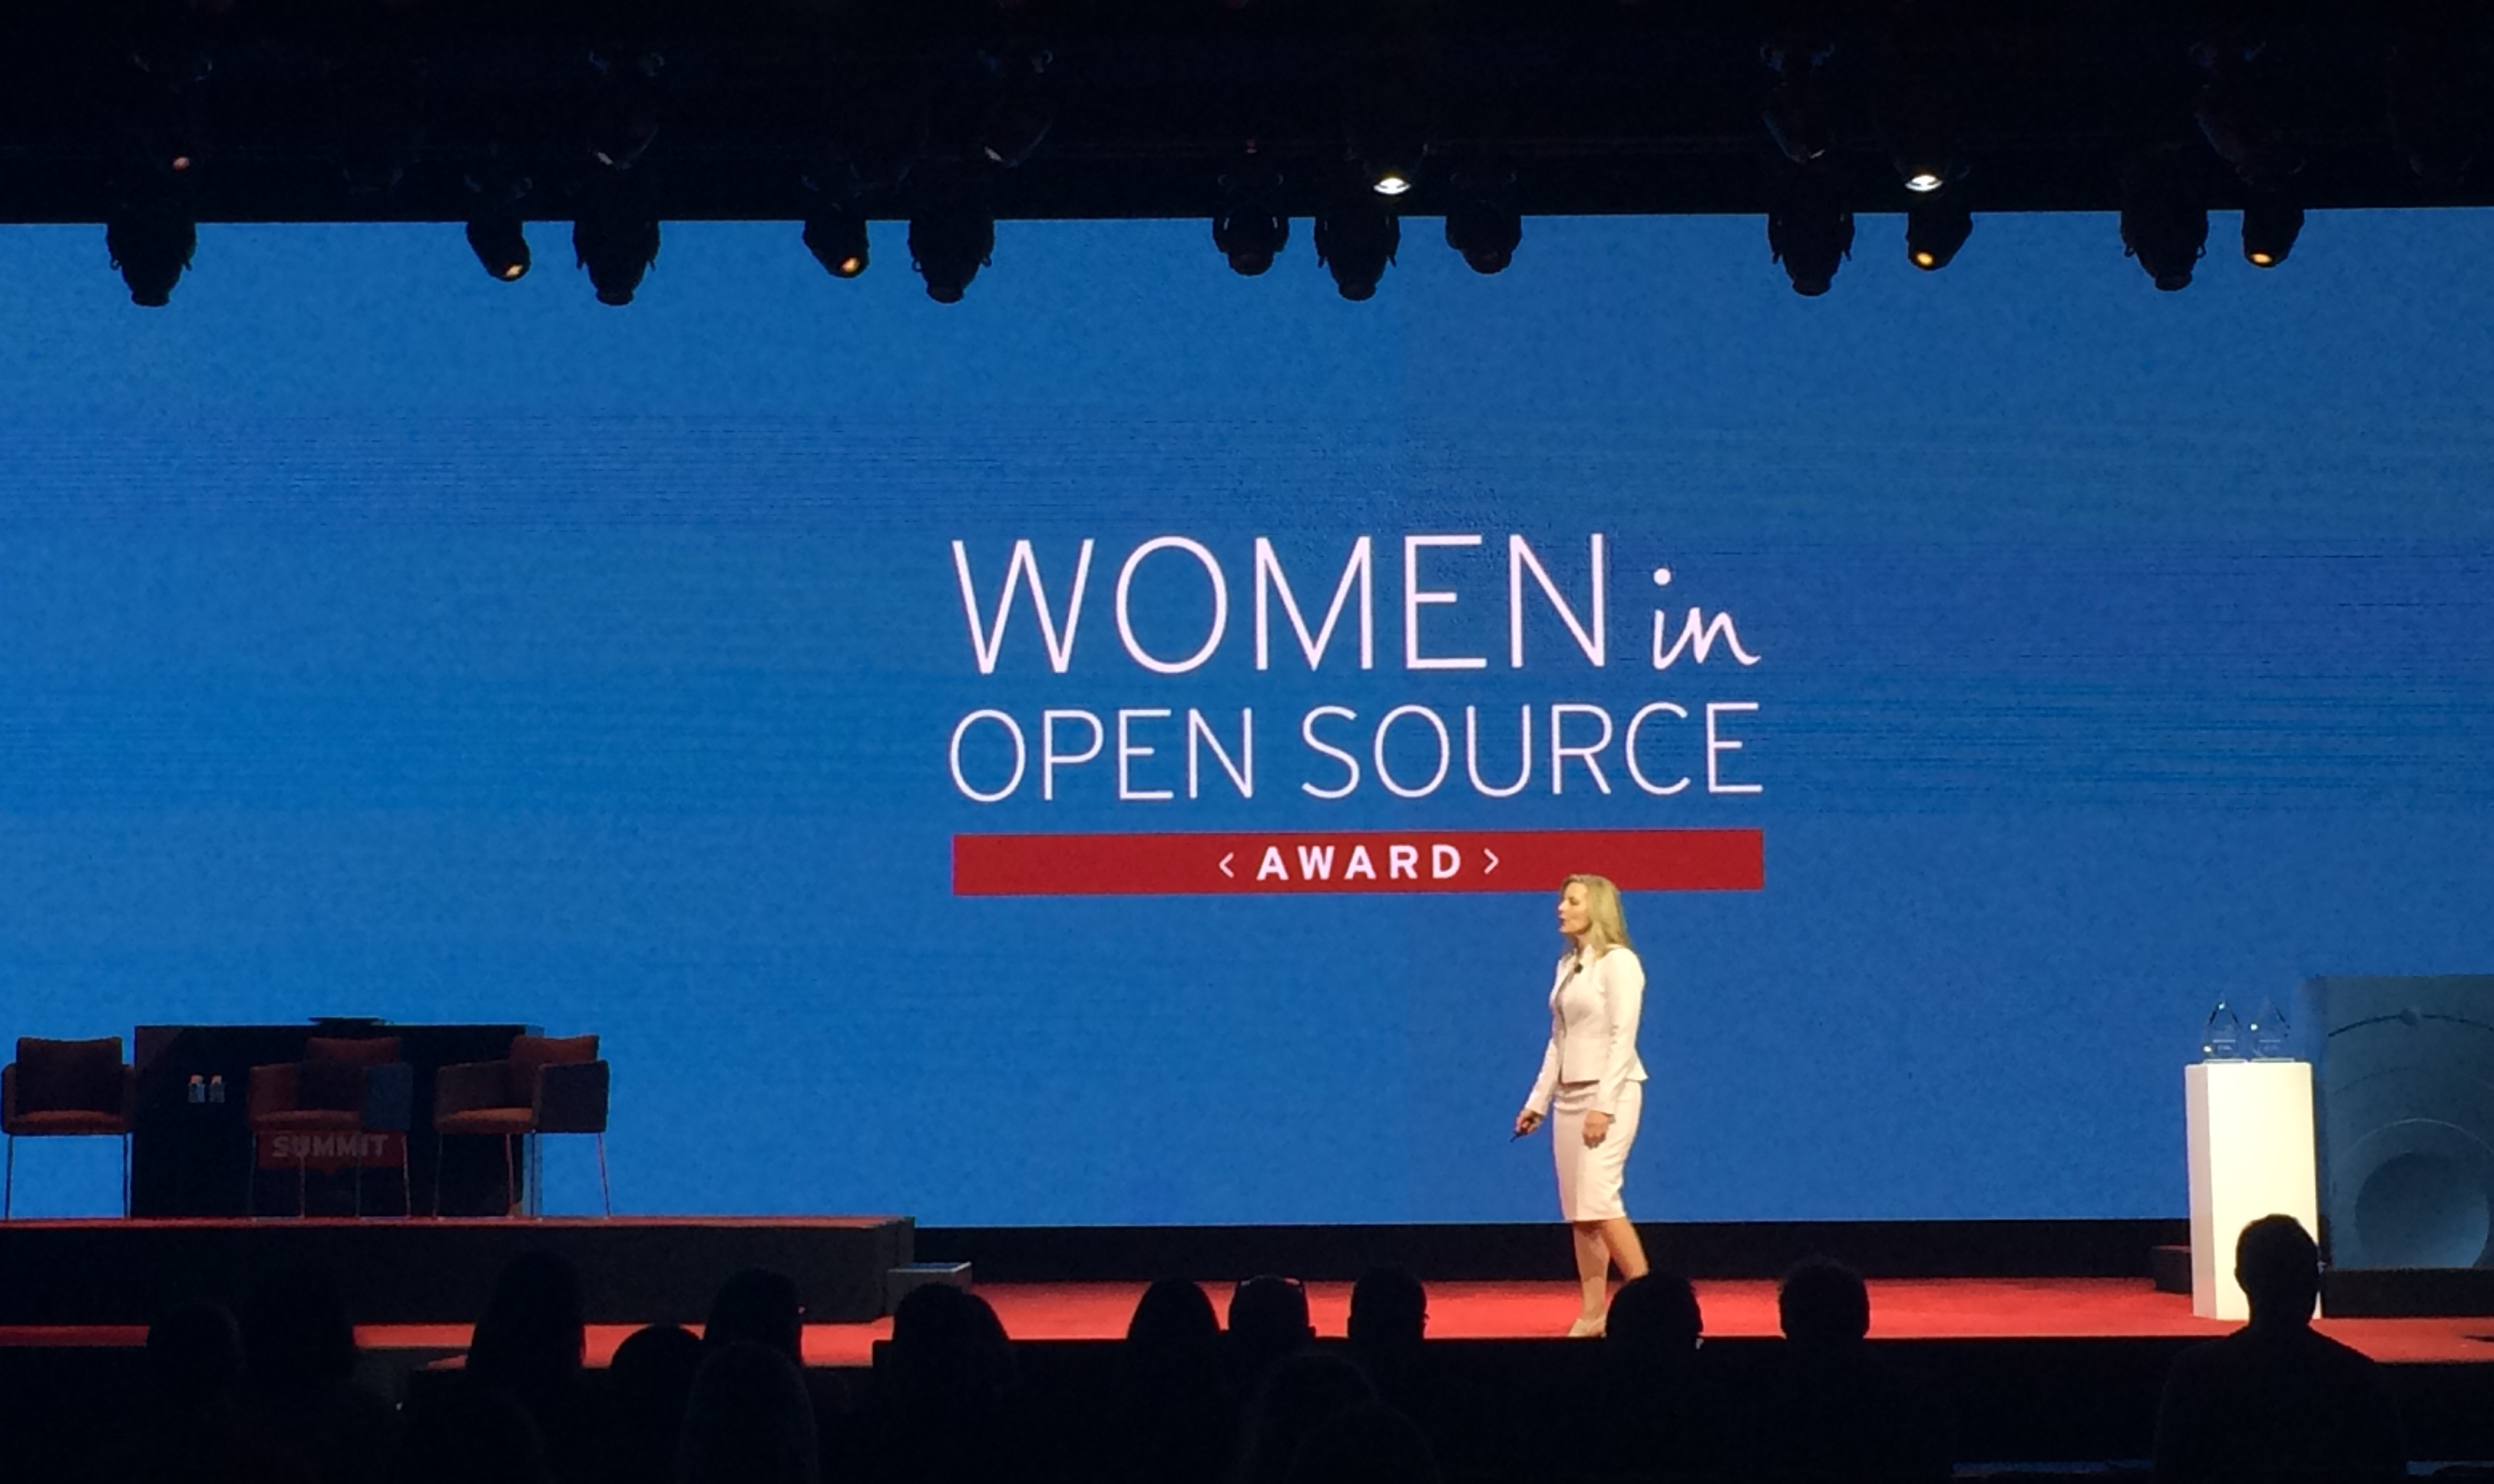
\includegraphics[scale=0.10]{wops.jpeg}
    \end{center}
Los premios son: 2.500 dólares de remuneración para usar como soporte de proyectos e iniciativas de código abierto, entrada gratuita, vuelo y alojamiento en hotel para la Red Hat Summit 2019 y
una ponencia como conferenciante destacada en un evento de Red Hat. De hecho en el futuro planeo participar en esta clase de eventos.\\
\textbf{Tiempo en leer el artículo y hacer la reseña: 30 minutos}

%Noviembre
\section*{Noviembre 2018}
Los dos artículos además del que cometaré que me llamaron la atención son:
\begin{itemize}
    \item PING: Richard Stallman en Valencia, Apache OpenOffice, Desktop Icons (GNOME Shell), Netflix a 1080p… - MuyLinux
    \item Fedora cumple 15 años - MuyLinux
\end{itemize}
\textbf{System76 presenta Thelio, sus nuevos PC de sobremesa - MuyLinux}
Thelio es una gama de computadoras, la idea principal que tenía System76 es que Thelio fuese construido puramente con hardware Open Source, sin embargo por las limitantes actuales, eso aún no ocurre, por ello tuvieron que hacer Thelio como una computadora cualquiera, lo que le hace especial es su diseño, es un CPU de madera, los componentes clave de estas máquinas siguen siendo lo de siempre: placa base, procesador, memoria y tarjeta gráfica de las principales marcas del mercado. Pero por algo se empieza y en lo que respecta a sus diseños, System76 ofrecerá también firmware abierto que está siendo certificado por OSHWA.

\begin{center}
    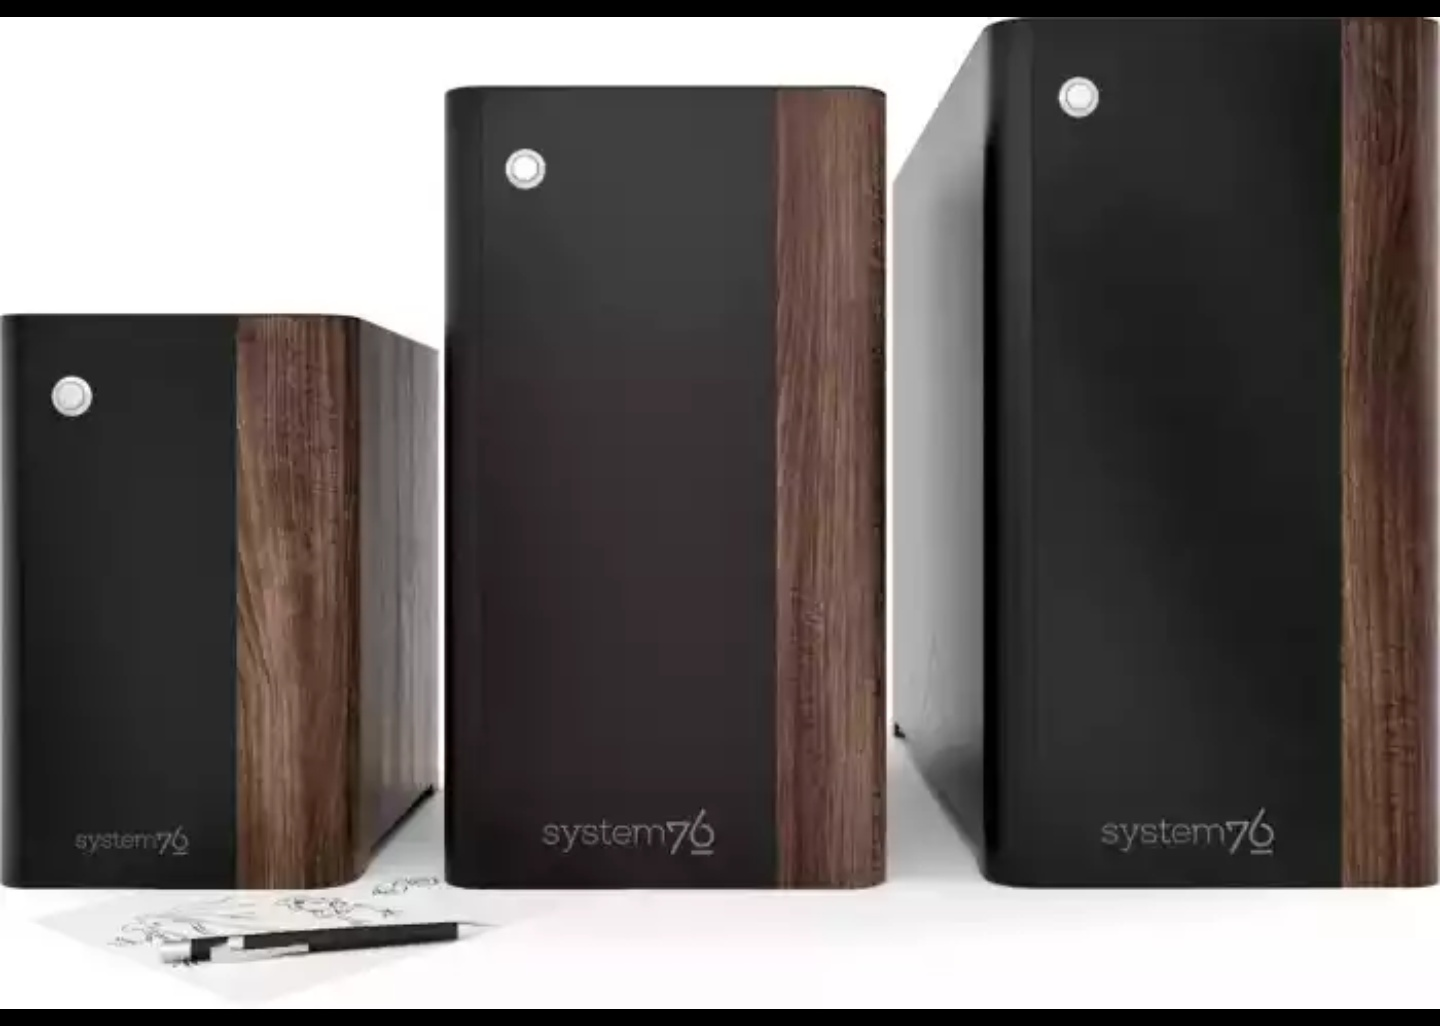
\includegraphics[scale=0.20]{thelio0.jpeg}
\end{center}
Hay 3 modelos distintos de Thelio:
\begin{itemize}
    \item Thelio\\
    Ryzen or Core CPUs\\
    Up to 32GB of Memory\\
    Radeon or GeForce GPUs\\
    Up to 24TB of Storage\\
    Space-Saving Design
    \item Thelio Major\\
    Threadripper or Core-X CPUs\\
    Up to 128GB of Memory\\
    Up to 4 GPUs\\
    Up to 46TB of Storage\\
    Maximum Configurability
    \item Thelio Massive\\
    Dual XEON CPUs\\
    Up to 768GB of ECC Memory\\
    Up to 4 GPUs\\
    Up to 86TB of Storage\\
    Epitome of performance
\end{itemize}

Me gustó esta nota, pues yo no conocía esta gama de computadoras y me parece un buen concepto que solo se quiera utilizar Hardware Open Source.\\
\textbf{Tiempo en leer el artículo y hacer la reseña: 30 minutos}
%Diciembre
\section*{Diciembre 2018}
Los dos artículos además del que cometaré que me llamaron la atención son:
\begin{itemize}
    \item Rest in Peace Fedora 27 - Full Circle - Página 4
    \item Red Hat Enterprise Linux come to Windows 10 in the Form WLinux Enterprise - Full Circle - Página 10
\end{itemize}
\textbf{Linux and Super Computers - Linux Journal - Página 79}\\
Éste artículo trata sobre la historia de la computación y de como fue el inicio de las súpercomputadoras, principalmente menciona a Seymour Cray, mismo que diseñó una máquina para la Agencia de Seguridad de las Fuerzas Armadas, que, solo unos pocos años antes (en 1949), fue creada para encargarse de actividades criptográficas y de inteligencia electrónica para el ejército de Estados Unidos. Esta nueva agencia necesitaba una máquina más poderosa. Esto dio lugar a Atlas II que tenía un peso de 19 toneladas, fue una de las primeras computadoras en utilizar la memoria RAM.

    \begin{center}
        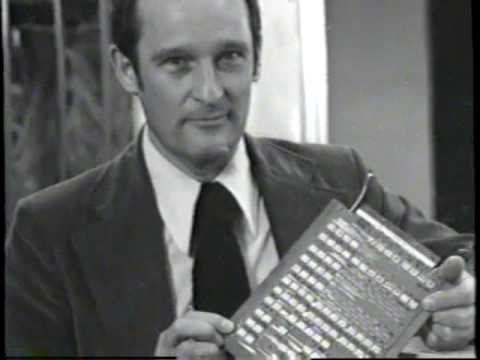
\includegraphics[scale=0.50]{seymour.jpg}
    \end{center}
    
Pero aquí no se detuvo, en 1952 Seymour Cray pidió permiso a "The Armed Forces Security Agency" para liberar y vender la computadora comercialmente, le dieron la autorización, pero tuvo que borrar instrucciones especiales, que consideraban que no debían estar al alcance de todo publico, ésta salió a la venta en 1953, con el nombre de UNIVAC 1103 que marco una nueva era para las Supercomputadoras. UNIVAC fue utilizada por la NASA y fue también un instrumento de desarrollo y diversas pruebas.\\
Hasta 1998 surgió la primera súpercomputadora que utilizaba como Sistema Operativo a Linux, conocida como el Cluster de Avalon, fue desarrollada en el Laboratorio Nacional de Los Álamos por un costo (comparativamente) muy pequeño de \$ 152,000. Compuesto por un grupo de computadoras DEC Alpha (68 núcleos en total) y con CPUs EV56 de 531MHz, esta bestia Linux-y generó la friolera de 19.3 Gigaflops, lo suficiente para ayudarlo a debutar como la 314 computadora más poderosa de la Tierra. Claro, llegar en el puesto 314 puede no parecer una victoria, ¡pero todos tienen que comenzar en algún lugar! Y en 1998, esto fue asombroso para la época. Cuando fue lanzada era una de las supercomputadoras más baratas de ese momento. También se menciona que en la actualidad todas las Súpercomputadoras que son muy veloces tienen como sistema operativo a Linux y que dificilmente será reemplazado por algún otro Sistema Operativo para las Súpercomputadoras. El Artículo me pareció muy interesante pues pocas veces nos interesamos en conocer el pasado de la actual tecnología con la que contamos, muchas veces ni siquiera conocemos a los autores que nos han brindado las bases para el avance tecnológico que tenemos hoy en día.\\
\textbf{Tiempo en leer el artículo y hacer la reseña: 45 minutos}

%Enero
\section*{Enero 2019}
Los dos artículos además del que cometaré que me llamaron la atención son:
\begin{itemize}
    \item Raspberry Pi’s New Compute Module 3+ is 10x Faster, Still Just as Cheap - OMG! Ubuntu!
    \item New Dell XPS 13 Developer Edition Goes on Sale Powered by Ubuntu - OMG! Ubuntu!
\end{itemize}
\textbf{El Gobierno de Corea del Sur apuesta por Linux para reemplazar a Windows - MuyLinux}\\
El Gobierno de Corea del Sur migrará todos sus equipos informáticos de Windows a Linux, según declaraciones del ministro del Interior y Seguridad del país. Me parece que es una noticia muy importante, pues al final Windows es Desarrollado en Estados Unidos y de alguna manera es depender de ellos para actualizaciones del sistema, cuando se trata de la seguridad de todo un país y datos que podrían comprometerse, lo mejor es utilizar Linux pues es más confiable. Creo que poco a poco Linux va ganando terreno ante el monstruo que es Windows. "Corea del Sur sería el segundo gran país asiático en tomar la decisión de migrar de Windows a Linux, después de que China anunciase lo propio para 2020 en detrimento de Windows XP, si bien no está del todo claro si se acabará cumpliendo. En cualquier caso, se trata de una noticia importante y la experiencia que se extraiga del proceso, de su desarrollo y resultado podrán servir de ejemplo a otros países."\\
\textbf{Tiempo en leer el artículo y hacer la reseña: 25 minutos}

%Febrero
\section*{Febrero 2019}
Los dos artículos además del que cometaré que me llamaron la atención son:
\begin{itemize}
    \item HITMAN viene a Linux y SteamOS el 16 de febrero - Linux Adictos
    \item GNOME 3.32 entra beta, la versión final llega el 13 de marzo - MasLinux
\end{itemize}
\textbf{El Parlamento asturiano vota a favor propuesta de fomento del software libre - MasLinux}
\begin{quote}
    El software libre es una cuestión transversal y de interés general, como demuestra el abanico de partidos políticos que han apoyado la propuesta parlamentaria. Las ventajas del software libre, que van desde la seguridad (permitir realizar auditorías de seguridad, algo imposible con el software no libre) hasta el económico (dado que el software libre se define por impedir que el vendedor bloquee el código y por tanto el fenómeno del “cliente cautivo” o “consumidor cautivo” que lastra el buen funcionamiento de la administración y la eficiencia del gasto debido a la costosa dependencia obligada respecto a una única empresa que concentra un gran poder en situación de monopolio), han sido razones fundamentales para el apoyo de la propuesta parlamentaria y para promover ahora su materialización práctica. Ninguna empresa es excluida por incluir la condición de ser software libre en las licitaciones y concursos públicos, y permite avanzar de una economía basada en la compra como fin último a una economía basado en servicios que satisfacen a empresas y administraciones, puesto que el software libre permite que si la empresa ganadora del concurso o licitación no presta un buen servicio cualquier otra empresa pueda tomar el relevo sin ninguna dificultad, lo cual no pasa con el software no libre actualmente usado en el que tras la compra personas y administraciones pública quedan encadenados de por vida como “clientes cautivos” a la empresa que en régimen de monopolio vende el software. El software libre, cuya historia se remonta al propio comienzo de la informática personal hace 35 años, ofrece actualmente alternativas maduras y profesionales en la gran mayoría de los ámbitos informáticos, siendo la elección de preferencia en muchas aplicaciones en las cuales la estabilidad y la seguridad son críticos. Un gran número de empresas ejemplifican el gran poder del software libre en el mundo empresarial, además la fiabilidad y robustez del software libre se demuestra por su predominio en sectores donde los aspectos técnicos predominan: desde el acelerador de partículas europeo hasta la propia infraestructura de Internet.
\end{quote}
Es sumamente importante esta clase de acontecimientos, porque en teoría esto nos da más libertad y de alguna manera permite mejorar la seguridad de nuestros datos, pocos gobiernos se atreven a promover el software libre, por ello esta noticia me pareció interesante.\\
\textbf{Tiempo en leer el artículo y hacer la reseña: 30 minutos}

%Marzo
\section*{Marzo 2019}
Los dos artículos además del que cometaré que me llamaron la atención son:
\begin{itemize}
    \item NethServer Administrado Servicios - Atix Libre
    \item Bacula Backups Remotos - Atix Libre
\end{itemize}
\textbf{PSeint Pseudocódigo y Algoritmos - Página 1}\\
PSeint(Pseudocode, Interpreter) es un software pensado para que los programadores puedan desarrollar algoritmos computacionales por medio de pseudo código, con ello será más fácil que el programador se concentre en la parte lógica del programa, el principal atractivo de PSeint es justamente lo ya mencionado, pues el hecho de que te permita como programador concentrarte únicamente en la parte lógica del programa te permite despreocuparte por la parte más tecnica. Es muy sencilla la instalación de este software pues basta entrar a la página para encontrar el instalador para cualquier sistema operativo, hay muchos ejemplos de como se utiliza, además que en mi opinión personal, creo que sería muy útil para personas que apenas están adquiriendo experiencia en programación. No puedo escribir una reseña mucho más larga porque el artículo más que nada muestra ejemplos de la utilización de dicho software más el punto de vista personal del autor, sin embargo el tiempo que invertí además tiene que ver con que busqué por mi cuenta información sobre dicho software.
\begin{center}
    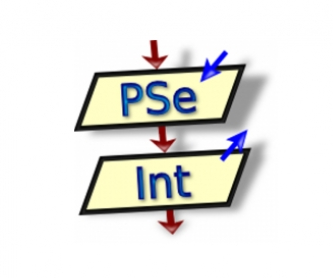
\includegraphics[scale=0.50]{pseint.png}
\end{center}
\textbf{Tiempo en leer el artículo y hacer la reseña: 40 minutos}

%Abril
\section*{Abril 2019}
Los dos artículos además del que cometaré que me llamaron la atención son:
\begin{itemize}
    \item Microsoft lanza Visual Studio Code como Snap - MuyLinux
    \item OpenProject Gestión de Proyectos - Atix Libre
\end{itemize}
\textbf{DataScience Plataformas OpenSource - Atix Libre}\\
Este artículo habla sobre machine learning principalmente y analiza a profundidad la ciencia de datos.
LaCiencia de Datos se compone según el artículo por lo siguiente:
\begin{itemize}
    \item La ciencia de datos es la disciplina que involucra métodos científicos, procesos y
    sistemas para extraer conocimiento o un mejor entendimiento de datos en sus diferentes
    formas, ya sea estructurados o no estructurados.
    \item La ciencia de datos es la disciplina de hacer que los datos sean útiles
    \item La ciencia de datos es el estudio de dónde proviene la información, qué representa y
    cómo se puede convertirse en un recurso de gran valor para las empresas o
    instituciones al momento de de formular estrategias y toma de decisiones.
\end{itemize}
Además de lo anterior nos encontramos con que hay varios tipos de análisis de datos:
\begin{itemize}
    \item Muchas veces hacemos referencia al análisis de datos, pero no conocemos los diferentes tipos
    que existen, aquí alguna descripción de los mismos:
    \item Descriptivo: Este tipo de análisis se centra en describir un conjunto de datos.
    \item Exploratorio: Su objetivo es encontrar relaciones entre los datos que no se conocían
    previamente.
    \item Inferenciales: Se hace uso de los datos de una muestra dentro una población mas
    grande para poder generalizar el comportamiento de la misma a partir de la muestra.
    \item Predictivas: Permite hacer uso de los datos sobre cierto objeto o fenómeno para
    predecir los valores de otro fenómeno u objeto.
    \item Causales: Trata de encontrar que pasa con una variable dentro un modelo si se varían
    otros parámetros.
    \item Mecanistas: Aunque es muy raro este tipo de análisis, este trata de entender los
    cambios exactos de las variables que producen en otras variables, para esto es
    necesario 
\end{itemize}
 Una ventaja de la ciencia de datos es que podemos ordenar y manejar grandes cantidades de información, lo cual hace más sencilla su manipulación, la única desventaja como siempre es que no todo el mundo sabe manejar bases de datos y solo las personas con suficiente experiencia y amplios conocimientos podrán hacer un trabajo óptimo. El software del que se habla en el artículo es Anaconda, el cual es muy bueno, es código abierto, multiplataforma, Interfáz web, Machine Learning, visualización de datos, consola entre otras herramientas.
 \vfill
 \begin{center}
     
\includegraphics[scale=0.40]{anaconda.png}
     
\includegraphics[scale=0.30]{DataS.png}
 \end{center}
 \textbf{Tiempo en leer el artículo y hacer la reseña: 1hr}

%Mayo
\section*{Mayo 2019}
Los dos artículos además del que cometaré que me llamaron la atención son:
\begin{itemize}
    \item Stack Overflow Compromised - Admin Magazine
    \item Scientists Simulate One Billion Atoms to Model a Gene of DNA
\end{itemize}
\textbf{New Class of CPU Flaws Affect Almost Every Intel Processor Since 2011 - Admin Magazine}
Esta noticia me llamó la atención pues actualmente stackoverflow es de los sitios más utilizados por programadores, tengo entendido que hay varios niveles de usuario dependiendo de la partición, además de que pueden guardar información personal, como información de su area laboral, o la bolsa de trabajo que les interesa, por ello se me hace muy grave que durante una semana mantuvieran cautiva la página, pero el equipo de trabajo de stackoverflow al final triunfo y pudieron tener el control nuevamente sobre el sitio web. Al final lo único que pronunció el equipo de trabajo de stackoverflow fue: Como parte de nuestros procedimientos de seguridad para proteger los datos confidenciales de los clientes, mantenemos una infraestructura y redes separadas para los clientes de nuestros productos de Equipos, Negocios y Empresas, y no hemos encontrado evidencia de que se haya accedido a esos sistemas o datos de clientes. Nuestros negocios de Publicidad y Talento Tampoco fueron impactados por esta intrusión.

\begin{center}
    
\includegraphics[scale=0.40]{stack.png}
\end{center}
\textbf{Tiempo en leer el artículo y hacer la reseña: 20 minutos}
\end{document}